\chapter{Model dyskretny}
\section{Transmitancja}
\section{Równania stanu}
\section{Porównanie modelu dyskretnego i ciągłego}
\begin{figure}
	\centering
	\includegraphics[width=.8\linewidth]{plot/dysk_1.eps}
	\caption{Porównanie modelu ciągłego i dyskretnego dla czasu próbkowania 0.1 min}
	\label{fig:dys01}
\end{figure}
\begin{figure}
\centering
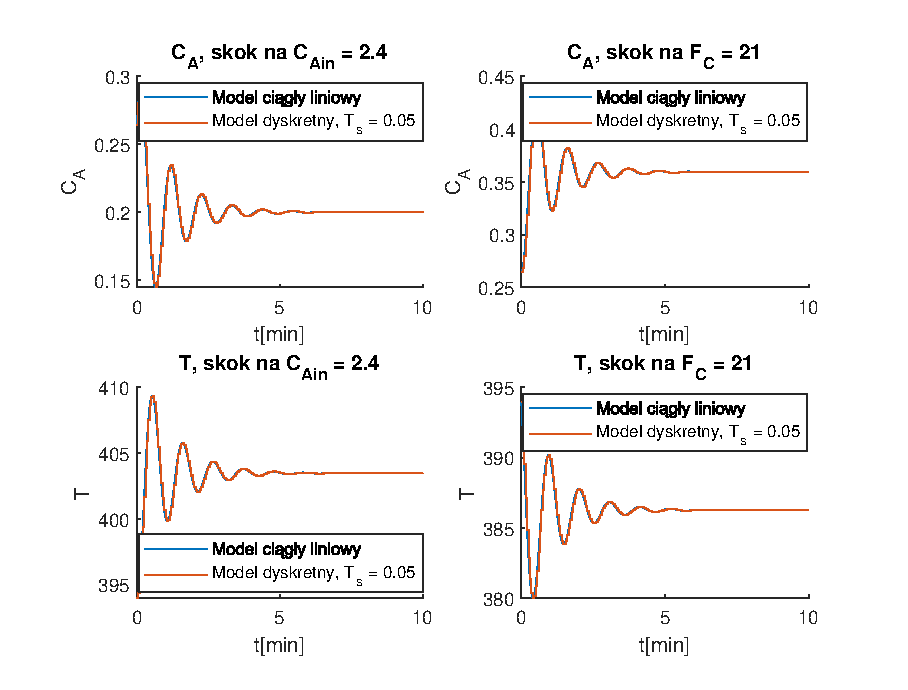
\includegraphics[width=.8\linewidth]{plot/dysk_05.eps}
\caption{Porównanie modelu ciągłego i dyskretnego dla czasu próbkowania 0.05 min}
\label{fig:dys005}
\end{figure}
\begin{figure}
\centering
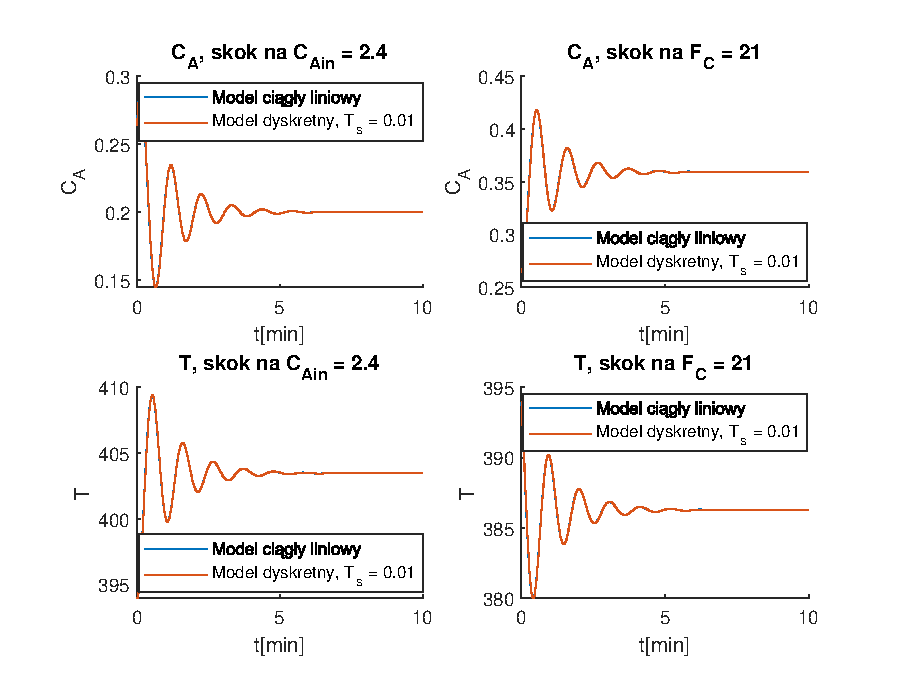
\includegraphics[width=.8\linewidth]{plot/dysk_01.eps}
\caption{Porównanie modelu ciągłego i dyskretnego dla czasu próbkowania 0.01 min}
\label{fig:dys001}
\end{figure}